%--------------------导言--------------------%
\documentclass{report}
\usepackage{xcolor}
\usepackage{fancyhdr}%导入fancyhdr包
\usepackage{ctex}%导入ctex包
\usepackage{graphicx}
\pagenumbering{Roman}%设置页码格式,大写字母标页
\pagestyle{fancy}
\fancyhead[L]{}
\fancyhead[R]{\textcolor{gray}{课程实验}}
\fancyhead[L]{\textcolor{gray}{《深度学习》}}
\fancyfoot[L]{\textcolor{gray}{北京理工大学}}
\fancyfoot[C]{\thepage}
\fancyfoot[R]{\textcolor{gray}{计算机学院}}
\renewcommand{\headrulewidth}{0.4pt}%分隔线宽度4磅
\renewcommand{\footrulewidth}{0.4pt}
\usepackage{setspace}
\setstretch{1.2}



%--------------------正文--------------------%
\begin{document}
	\begin{titlepage}
		\begin{center}
			\setstretch{1.5} % 设置行间距为1.5倍
			{\LARGE \textbf{2021-2022学年第2学期\\《深度学习》\\课程实验报告\\ \quad \\ \textbf{实验一:基于全连接网络的手写数字识别}}}\\[2cm]
			{\Large 姓名:XXX \qquad 学号:XXXXXXXXX}\\[1cm]
			{\Large 2023年3月13日}\\[2cm]
		\end{center}
	\end{titlepage}

	\section{实验目的}
	本次实验通过配置conda环境以及pytorch深度学习环境,使学生了解相关知识。并通过让学生自行从原始数据构建自定义数据集和使用pytorch搭建简单的手写数字识别全连接网络,使学生能够学习到pytorch深度学习框架的基础知识,并了解其训练和验证的全过程。
	
	\section{实验内容}
	\begin{enumerate}
		\item 使用原始图片和标签数据,构建自定义的手写数字识别数据集。
		\item 搭建合适的全连接网络用于手写数字图片分类。
		\item 对模型进行训练,训练完成之后对测试集进行预测,并生成预测结果文件。
	\end{enumerate}
	
	
	\section{实验原理}
	\subsection{概述}
	MNIST手写数字识别是计算机视觉领域中的一个经典问题,它的目标是将一张包含手写数字的图像作为输入,输出该图像所代表的数字。全连接网络是其中一种实现手写数字识别的算法。
	
	全连接网络是由多个全连接层组成的神经网络。在全连接层中,每个神经元都与上一层中的所有神经元相连,每个连接都有一个权重。给定一个输入向量,网络通过将输入向量与每个神经元的权重相乘,然后将结果相加并通过激活函数进行转换来计算下一层的输出向量。
	
	在MNIST手写数字识别问题中,每张图像都有28x28个像素点,可以将每个像素点看作输入向量中的一个元素。全连接网络将这些输入向量作为输入,并经过多个全连接层的计算,最终输出一个长度为10的向量,其中每个元素表示该图像所代表的数字的概率。通过比较这个向量中概率最大的元素与图像真实的标签,可以得出网络的正确率。
	
	在实现全连接网络时,通常使用反向传播算法进行训练。该算法通过计算损失函数关于网络中所有参数的梯度,并使用梯度下降算法来更新这些参数,以使损失函数最小化。
	
	
	\subsection{交叉熵损失函数}
	交叉熵损失函数(Cross-entropy loss function)是一种常用的深度学习模型的损失函数,通常用于分类问题中。其主要思想是利用目标标签和模型的预测标签之间的差距来度量模型预测的准确性,并且在训练过程中通过优化损失函数来调整模型参数,从而提高模型的预测准确性。
	
	交叉熵损失函数的定义是基于信息论中的交叉熵概念。在分类问题中,交叉熵损失函数可以表示为:
	
	$$J=-\frac{1}{N}\sum_{i=1}^{N}\sum_{k=1}^{K}y_{ik}\log{\hat{y}_{ik}}$$
	
	其中,$N$表示样本数量,$K$表示类别数量,$y_{ik}$是第$i$个样本的第$k$个标签值(0或1),$\hat{y}_{ik}$是第$i$个样本在第$k$个类别上的预测概率值。在训练过程中,我们将真实标签值表示为一个one-hot向量,即只有正确标签所在的位置为1,其他位置为0。
	
	交叉熵损失函数的本质是利用了信息熵的概念来度量模型预测的不确定性和目标标签的真实信息量之间的距离。具体来说,当模型预测正确时,交叉熵损失函数值趋近于0;当模型预测错误时,交叉熵损失函数值趋近于无穷大。因此,在训练过程中,我们通过不断调整模型参数来最小化交叉熵损失函数,从而提高模型的预测准确性。
	
	交叉熵损失函数是深度学习中常用的一种损失函数,主要用于分类问题中。其本质是基于信息论的交叉熵概念,通过度量模型预测的准确性来调整模型参数,从而提高模型的预测准确性。
	
	\subsection{随机梯度下降}
	随机梯度下降算法(Stochastic Gradient Descent,简称SGD)是一种用于优化模型参数的常见算法,特别适用于大规模数据集和深度学习模型。其主要思想是利用每个训练样本的梯度信息来更新模型参数,从而逐步降低目标函数的损失值。
	
	具体来说,SGD算法的步骤如下:
	
	\begin{enumerate}
		\item 初始化模型参数,例如权重和偏置值等。
		\item 随机从训练集中选择一个样本,计算该样本的梯度值。
		\item 使用梯度下降算法更新模型参数,即按照一定的学习率和梯度值方向更新参数。
		\item 重复步骤2-3,直到达到一定的迭代次数或者满足一定的收敛条件。
	\end{enumerate}
	
	与传统的批量梯度下降算法(Batch Gradient Descent,简称BGD)相比,SGD算法每次只使用一个样本来计算梯度和更新参数,因此其收敛速度更快,尤其适用于大规模数据集和高维模型。同时,由于SGD算法对于每个样本的梯度计算和参数更新是独立的,因此可以很方便地在分布式环境下进行并行计算。
	
	然而,SGD算法也存在一些缺点。由于每个样本的梯度计算是随机的,因此可能会引入噪声和不稳定性,导致收敛效果不佳。为了解决这个问题,通常会采用一些变种的随机梯度下降算法,例如带动量的随机梯度下降(Momentum SGD)、自适应学习率的随机梯度下降(Adagrad、Adadelta、Adam等)等。

	
	\section{实验过程}
	\subsection{实验环境配置}
	\begin{enumerate}
		\item 本地验证环境
		\begin{table}[htbp]
			\caption{本地验证环境}
			\centering
			\renewcommand{\arraystretch}{1.5}
			\begin{tabular}{|c|ccc|}
				\hline
				操作系统                       & \multicolumn{1}{c|}{Windows11 专业版}                    & \multicolumn{1}{c|}{硬件环境}                 & CUDA 11.1            \\ \hline
				深度学习框架                     & \multicolumn{1}{c|}{PyTorch 1.10.1+cu113}             & \multicolumn{1}{c|}{Python版本}             & 3.8.10               \\ \hline
				\multicolumn{1}{|l|}{运行说明} & \multicolumn{3}{l|}{\begin{tabular}[c]{@{}l@{}}直接右键运行,或使用命令"python Exp1-HandWritingNumRec.py"\\ (参数已设置默认值)\end{tabular}} \\ \hline
			\end{tabular}
		\end{table}
	
		\item 云环境
		\begin{table}[htbp]
			\caption{云环境}
			\centering
			\renewcommand{\arraystretch}{1.5}
			\begin{tabular}{|c|ccc|}
				\hline
				云平台                       & \multicolumn{1}{c|}{Colab}                    & \multicolumn{1}{c|}{硬件环境}                 & CUDA 12.0            \\ \hline
				深度学习框架                     & \multicolumn{1}{c|}{PyTorch 1.13.1+cu116}             & \multicolumn{1}{c|}{Python版本}             & 3.8.10               \\ \hline
				\multicolumn{1}{|l|}{运行说明} & \multicolumn{3}{l|}{\begin{tabular}[c]{@{}l@{}}运行shell脚本"run.sh"
				\end{tabular}} \\ \hline
			\end{tabular}
		\end{table}
	
	
	\end{enumerate}
	\subsection{自定义数据加载器}
	本实验中实现了一个用于加载手写数字识别数据集的类,该类继承自PyTorch的Dataset类。该数据集由一组图片和对应的标签组成,其中图片保存在data\_root指定的路径下的images文件夹中,标签可以通过label\_name指定的txt文件读取得到。
	
	在\_\_init\_\_函数中,类的实例化会自动调用该函数进行初始化。在该函数中,首先将数据集根目录、图片数据和标签数据分别保存在类的属性data\_root、images和labels中。然后遍历images文件夹中的所有图片文件,按文件名的数字顺序排序后逐一读入,并将读入的图像数据以numpy数组的形式保存在images属性中。如果label\_name为None,则将labels属性初始化为0,否则从指定的txt文件中读入标签数据,并将其以列表的形式保存在labels属性中。
	
	\_\_getitem\_\_函数用于获取指定索引的数据和标签。该函数首先从images和labels属性中获取对应索引的图像和标签,然后将图像数据转换成PyTorch张量并返回图像数据和标签数据的元组。
	
	最后,实现\_\_len\_\_函数返回数据集的大小,即数据集中包含的图像数量。
	
	具体编码如图\ref{fig:data}所示。
	
	
	\subsection{模型定义}
	本实验实现了一个手写数字识别的神经网络模型的实现。这个神经网络继承自PyTorch中的nn.Module类,用于封装神经网络的结构和前向传播函数。
	
	在网络的初始化函数\_\_init\_\_()中,首先调用父类的初始化方法来创建一个空的神经网络模型。接着通过实例化nn.Linear对象定义了三个全连接层,分别为输入层(fc1)、隐藏层(fc2)、输出层(fc3),其输入和输出节点数分别为28 $\times$ 28 $\times$ 3和512、256、10。这里28 $\times$ 28 $\times$ 3是因为手写数字图像是28 $\times$ 28像素,而每个像素点有RGB三个通道,因此输入层的节点数为28 $\times$ 28 $\times$ 3。
	
	在模型的前向传播函数forward()中,首先使用view()函数将输入的图像数据x展开成一维向量形式,并送入输入层(fc1),随后使用ReLU激活函数对隐藏层(fc2)进行激活,再将激活后的结果送入输出层(fc3),得到最终的输出结果。最后将输出结果作为函数的返回值。
	
	图\ref{fig:model}为保存后的模型结构,这个神经网络模型的结构比较简单,只包含一个隐藏层,因此容易训练。
	
	\begin{figure}[htbp]
		\centering
		\begin{minipage}[t]{0.60\textwidth}
			\centering
			\centering
			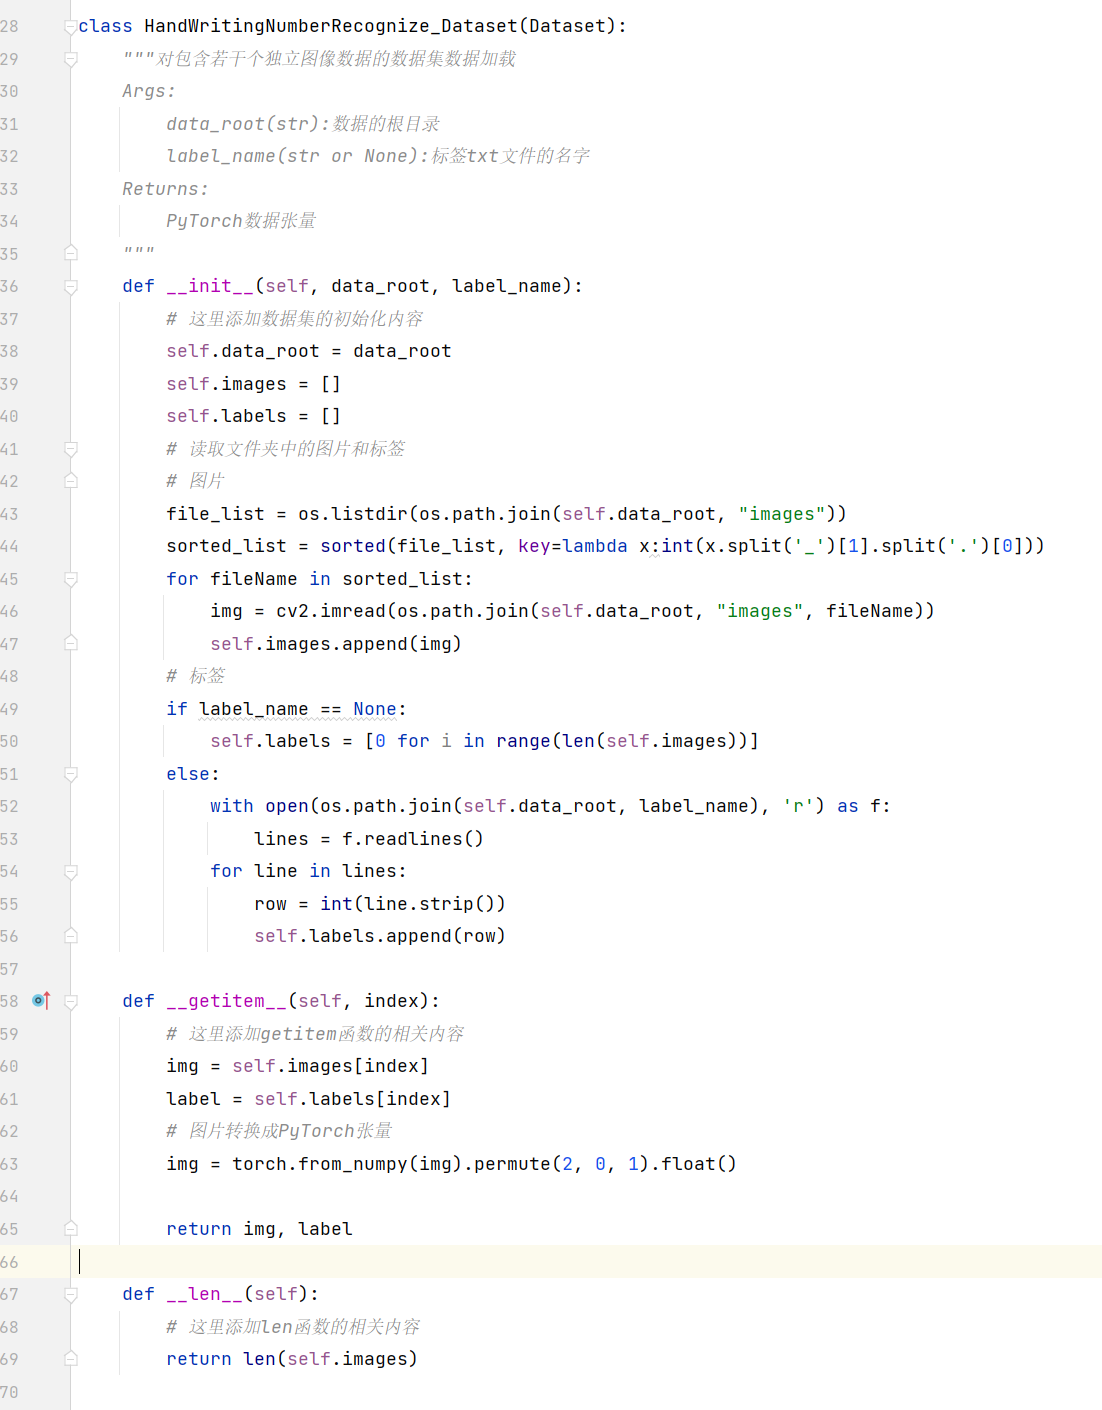
\includegraphics[width=0.8\textwidth]{fig/fig4.png}
			\caption{自定义数据加载器}
			\label{fig:data}
		\end{minipage}
		\hfill
		\begin{minipage}[t]{0.38\textwidth}
			\centering
			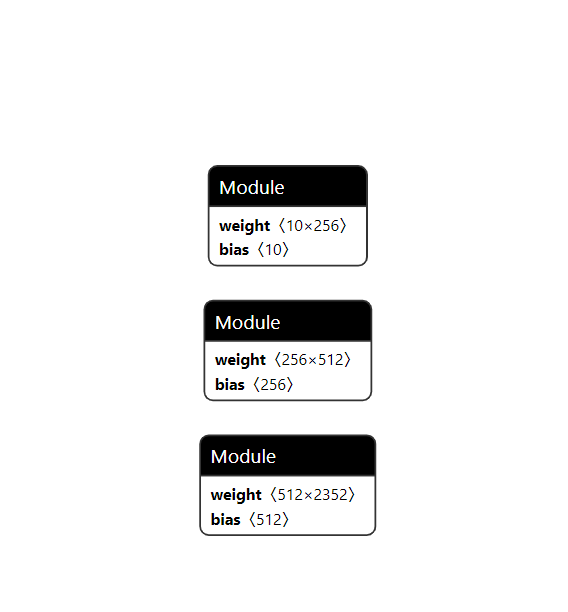
\includegraphics[width=0.9\textwidth]{fig/fig2.png}
			\caption{模型结构}
			\label{fig:model}
		\end{minipage}
	\end{figure}

	
	\subsection{学习率以及优化器和损失函数的选择}
	为了寻找最佳的一个适合模型的优化器和损失函数,实验中设置了一个shell脚本,用于在不同的优化器和损失函数下运行Python脚本。
	
	首先,脚本定义了两个数组:opt\_values和loss\_values。这些数组包含了不同的优化器和损失函数的名称。然后,使用两个嵌套的for循环迭代这些数组中的所有组合。在每个迭代中,脚本使用当前的opt和loss值来运行Python脚本"Exp1-HandWritingNumRec.py",并使用命令行参数将这些值传递给Python脚本。
	
	具体地说,"-opt"和"-loss"是Python脚本中定义的命令行参数,用于指定优化器和损失函数的名称。脚本将这些值传递给Python脚本,以便在每个迭代中使用不同的组合运行模型并记录结果。此脚本的目的在于“超参数优化”,旨在找到模型的最佳设置。
	
	最终,选择SGD + CrossEntropyLoss的组合作为本实验的优化器和损失函数。
	
	
	此外,学习率的大小对于一个模型也很重要。如果它太大,优化函数就会发散;如果它太小,训练就会需要过长时间,或者我们最终只能得到次优的结果。
	另外,衰减速率同样很重要。如果学习率持续过高,我们可能最终会在最小值附近弹跳,从而无法达到最优解。简而言之,我们希望速率衰减,但要比慢,这样能成为解决凸问题的不错选择。
	除了衰减速率,另一个同样重要的方面是初始化。这既涉及参数最初的设置方式,又关系到它们最初的演变方式。这被戏称为预热(warmup),即我们最初开始向着解决方案迈进的速度有多快。一开始的大步可能没有好处,特别是因为最初的参数集是随机的。最初的更新方向可能也是毫无意义的。
	
	本实验的模型设置以及数据较为简单,采用固定的学习率也能很快收敛。本实验设置学习率为0.001。
	
	\subsection{实验日志}
	运行代码时,程序会自动将输出保存到log日志中。
	
	\section{实验结果与分析}
	\subsection{结果}
	几种优化函数的效果对比如图\ref{fig:contrast}所示,选择SGD + CrossEntropy的实验运行结果如截图\ref{fig:result}所示。
	
	\begin{figure}[htbp]
		\centering
		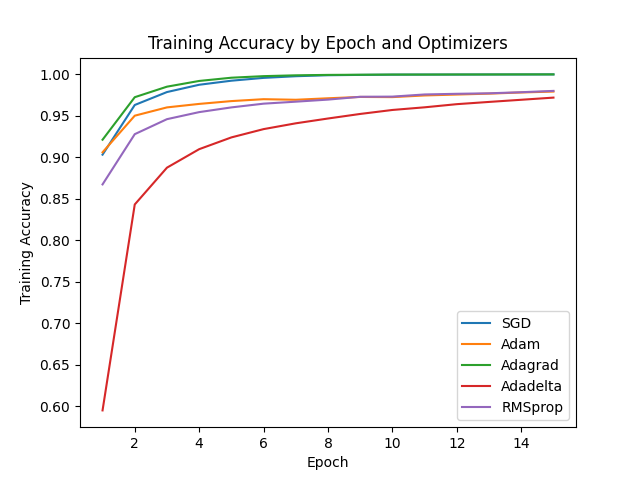
\includegraphics[width=1.\textwidth]{fig/fig3.png}
		\caption{几种优化函数的对比}
		\label{fig:contrast}
	\end{figure}
	
	\begin{figure}[htbp]
		\centering
		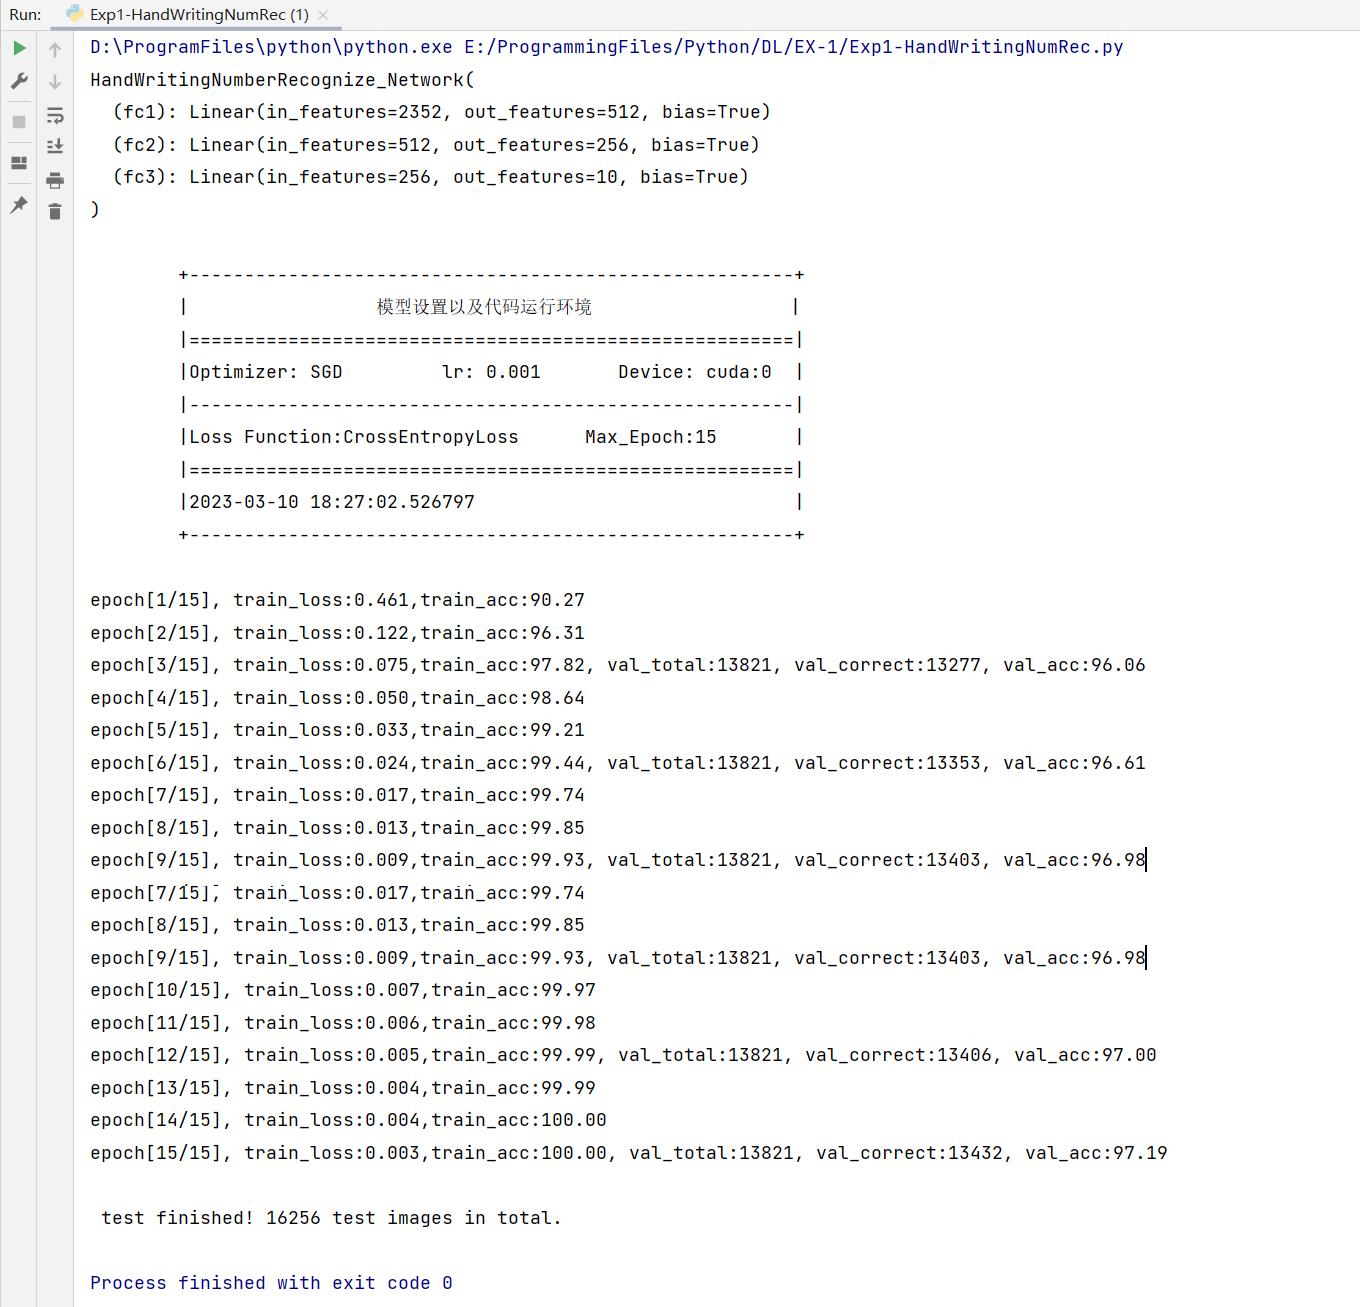
\includegraphics[width=1.2\textwidth]{fig/fig1.png}
		\caption{实验运行结果}
		\label{fig:result}
	\end{figure}
	
	\subsection{出现的问题及分析}
	
	\begin{enumerate}
		\item 首次实验时,出现训练中训练准确率增长很慢乃至不增长,验证集的准确率一直不增长,大致稳定在9.0\% 至 11.0\%之间。经助教老师提醒,造成此类现象的原因是读取数据集时需要对文件先按照编号进行排序,才能使得图像和自己的标签相对应。
		
		\item 尝试搭配不同的优化器和损失函数,然而发现当使用例如MSELoss函数作为损失函数时,程序无法正常运行。经查,该函数常用于回归问题。本实验是多分类问题,显然使用交叉熵损失、负对数似然损失等更加合适。
	\end{enumerate}
	
	
	\section{心得 体会}
	通过本次实验,对全连接神经网络有了更清楚的认识。同时,也感受到了数据的正确性与科学性很重要。在文件不排序的情况下结果很“玄学”,说明了“近朱者赤,近墨者黑”,模型总能学习,但是学习到的规律可能与现实世界的规律背道而驰。
	
\end{document}





